%!TEX root = ../main.tex
\section{Integration Strategy} % (fold)
\label{sec:integration_strategy}

\subsection{Entry Criteria} % (fold)
\label{sub:entry_criteria}
% subsection entry_criteria (end)
To perform the integration tests the following task must be performed:
\begin{itemize}
	\item Design and check Unit Tests.
	\item Design and implements driver/stub classes and method.
	\item Design and create test data.
\end{itemize}

\subsection{Elements to be Integrated} % (fold)
\label{sub:elements_to_be_integrated}
All the components described in section 3 of the DD will have to be tested.
In detail:
\begin{itemize}
	\item \textbf{Server Component}:
	\begin{itemize}
		\item Queue Manager
		\item Ride Manager
		\item Actor Manager
		\item Position Manager
		\item Request Manager
		\item Database Interface
	\end{itemize}
	\item \textbf{User Client}
	\begin{itemize}
		\item Main Activity
		\item Signup Activity
	\end{itemize}
	\item \textbf{Driver Client}
	\begin{itemize}
		\item Driving Request Fragment
		\item Driving Activity
	\end{itemize}
\end{itemize}
% subsection elements_to_be_integrated (end)

\subsection{Integration Testing Strategy} % (fold)
\label{sub:integration_testing_strategy}
This plan will follow a bottom-up approach. Provided that the unit testing is completed, this strategy enables the integration to almost always use the actual code that will be deployed, allowing the testing team to hardly ever create stubs and mocks, and reduce the use of dummy code.
Of course this is not always possible and section \emph{\nameref{sec:program_stubs_and_test_data_required}} will specify when and what stubs are needed.
% subsection integration_testing_strategy (end)

\subsection{Sequence of Components} % (fold)
\label{sub:sequence_of_components}
The integration plan will follow this order:
\begin{enumerate}
	\item \nameref{ssub:server_component}
	\item \nameref{ssub:user_client}
	\item \nameref{ssub:driver_client}
	\item \nameref{ssub:client_server}
\end{enumerate}

The first three are needed in order to test the internal submodules. Once the first three test have taken place then it is possible to test the \emph{Client-Server} interaction, with both the \emph{User Client} and the \emph{Driver Client}.

% \begin{figure}[h!t]

% \centering
% \end{figure}

\begin{figure*}[h!t]
    \centering
    \caption{A graphic representation of the modules and interfaces that will be tested. Each arrow has a label assigned to it that identifies the integration test.}
	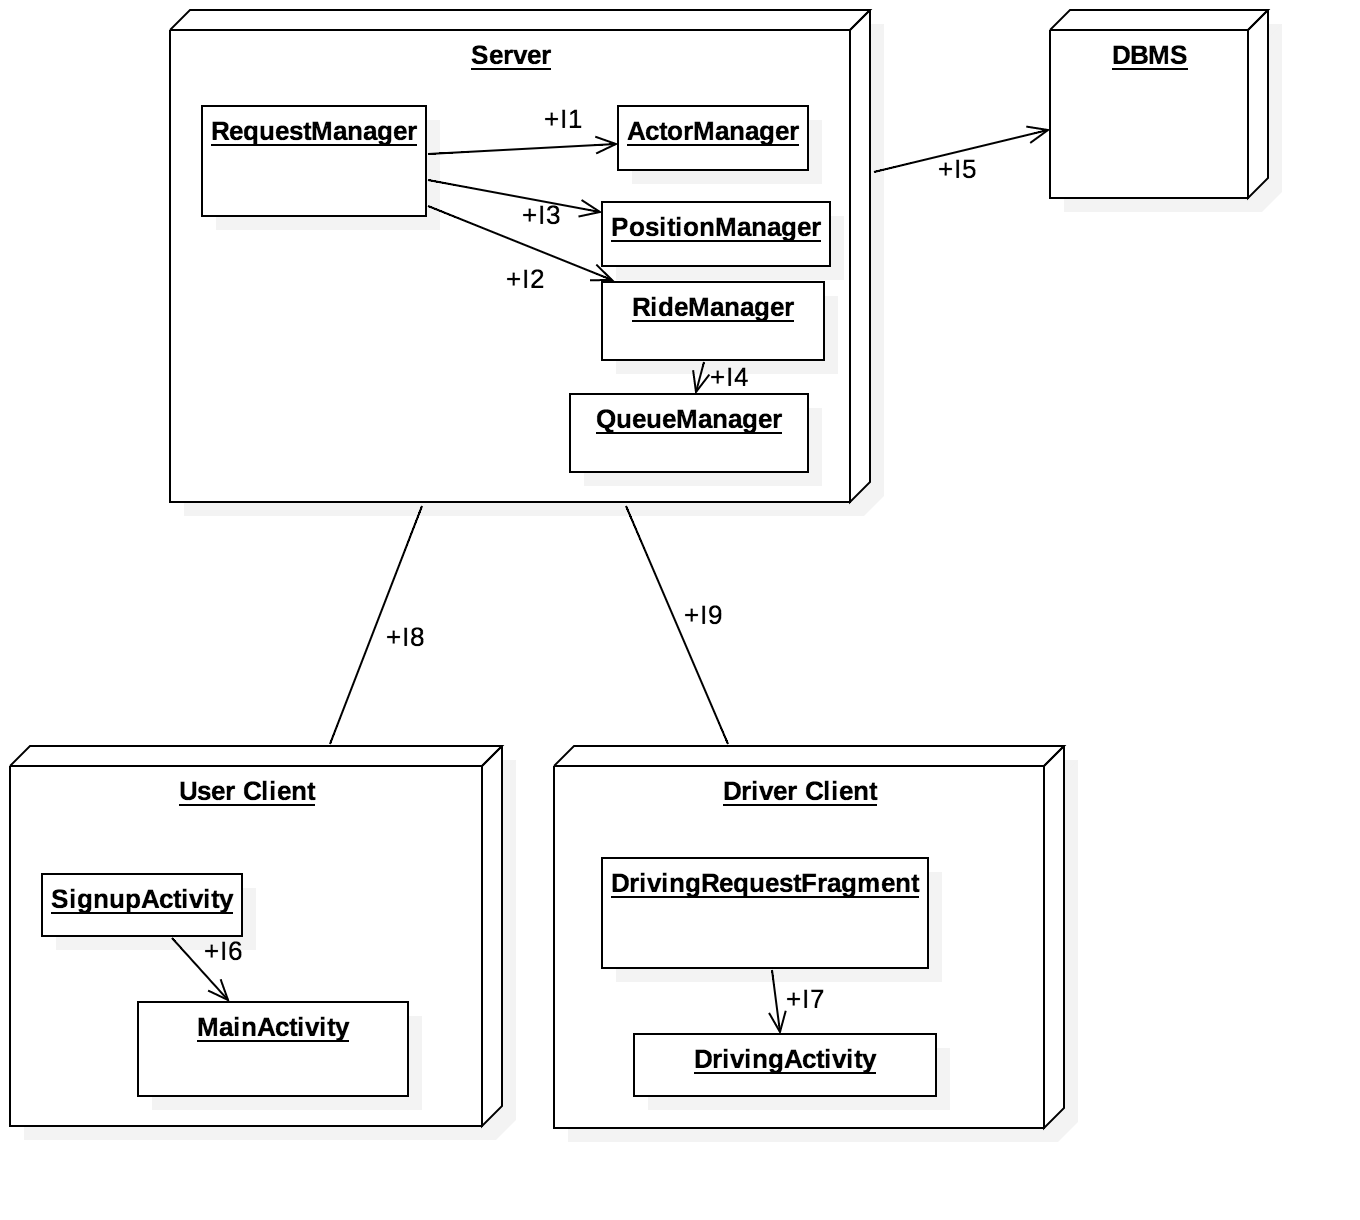
\includegraphics[width=\textwidth]{components}
\end{figure*}
\vfill
\clearpage

\subsubsection{Server Component} % (fold)
\label{ssub:server_component}

\begin{tabular} { p{20.0pt} | p{135pt} p{20pt} p{100pt} | p{60pt} } \hline
	\textbf{ID} & \multicolumn {3}{|c|}{\textbf{Integration Test}} & \textbf{Paragraphs} \\ \hline
	I1 & Request Manager & \textrightarrow & Actor Manager & 3.1 \\ \hline
	I2 & Request Manager & \textrightarrow & Ride Manager & 3.2 \\ \hline
	I3 & Request Manager & \textrightarrow & Position Manager & 3.3 \\ \hline
	I4 & Ride Manager & \textrightarrow & Queue Manager & 3.4 \\ \hline
	I5 & Database Interface & \textrightarrow & DBMS & 3.5 \\ \hline
\end{tabular}
% subsubsection server_component (end)

\subsubsection{User Client} % (fold)
\label{ssub:user_client}

\begin{tabular} { p{20.0pt} | p{135pt} p{20pt} p{100pt} | p{60pt} } \hline
	\textbf{ID} & \multicolumn {3}{|c|}{\textbf{Integration Test}} & \textbf{Paragraphs} \\ \hline
	I6 & Signup Activity & \textrightarrow & Main Activity & 3.6 \\ \hline
\end{tabular}
% subsubsection user_client (end)

\subsubsection{Driver Client} % (fold)
\label{ssub:driver_client}

\begin{tabular} { p{20.0pt} | p{135pt} p{20pt} p{100pt} | p{60pt} } \hline
	\textbf{ID} & \multicolumn {3}{|c|}{\textbf{Integration Test}} & \textbf{Paragraphs} \\ \hline
	I7 & Driving Request Fragment & \textrightarrow & Driving Activity & 3.7 \\ \hline
\end{tabular}
% subsubsection driver_client (end)

\subsubsection{Client-Server} % (fold)
\label{ssub:client_server}

\begin{tabular} { p{20.0pt} | p{135pt} p{20pt} p{100pt} | p{60pt} } \hline
	\textbf{ID} & \multicolumn {3}{|c|}{\textbf{Integration Test}} & \textbf{Paragraphs} \\ \hline
	I8 & User Client & \textrightarrow & Server & 3.8 \\ \hline
	I9 & Driver Client & \textrightarrow & Server & 3.9 \\ \hline
\end{tabular}

% subsubsection client_server (end)

% subsection sequence_of_components (end)

% section integration_strategy (end)